\chapter{Approach}\label{sec:approach}

Describe the main steps in your algorithm. An illustration is always helpful.\\

Here are some \LaTeX~tips:


\section{Headings}

  Your report can be structured using several different types of headings. Use the commands \textbackslash\texttt{chapter}\{.\}, \textbackslash\texttt{section}\{.\}, \textbackslash\texttt{subsection}\{.\}, and \textbackslash\texttt{subsubsection}\{.\}. Use the asterisk symbol \texttt{*} to suppress numbering of a certain heading if necessary, for example, \textbackslash\texttt{section*}\{.\}.


\section{References}\label{sec:references}

  References to literature are included using the command \textbackslash\texttt{cite}\{.\}. For example \cite{KleinMurray2007,Strasdat2010WhyFilter}. Your references must be entered in the file \texttt{bibliography.bib}. Making changes or adding new references in the bibliography file can be done manually or by using specialized software such as \textit{JabRef} which is free of charge.

  Cross-referencing within the text is easily done using \textbackslash\texttt{label}\{.\} and \textbackslash\texttt{ref}\{.\}. For example, this paragraph is part of chapter~\ref{sec:approach}; more specifically on page~\pageref{sec:references}.

\section{Writing Equations}\label{sec:math}

  The most common way to include equations is using the \texttt{equation} environment. Use \textbackslash\texttt{eqref}\{.\} to reference an equation, e.g. \eqref{eq:leastsquares}.
  \begin{equation}\label{eq:leastsquares}
      \begin{aligned}
        C(\mathbf{x}) &= \frac{1}{2} \ \sum_{i \in \mathcal I} \sum_{k \in \mathcal K_i} \mathbf{e}_{i,k}(\mathbf{x})^T \ \mathbf{W}_{i,k}  \ \mathbf{e}_{i,k}(\mathbf{x})  \\
        \hat{\mathbf{x}}^{LS} &= \text{argmin}_\mathbf{x} \ C(\mathbf{x}),
      \end{aligned}
  \end{equation}

  \begin{equation}\label{eq:se3}
    \mathtt{T}_i = \begin{bmatrix}\mathbf{R}_i & \mathbf{p}_i \\ 0 & 1\end{bmatrix} \qquad \text{with} \quad \mathbf{R}_i \in SO(3), \ \ \mathbf{p} \in \mathbb{R}^3.
  \end{equation}

\section{Including Graphics}\label{sec:epsgraph}
  The easiest way to include figures in your document is to use pdf figures if you use \texttt{pdflatex} to compile. Figure \ref{img:notation} was created with the use of the open source program \texttt{ipe}.

  \begin{figure}[h]
     \centering
     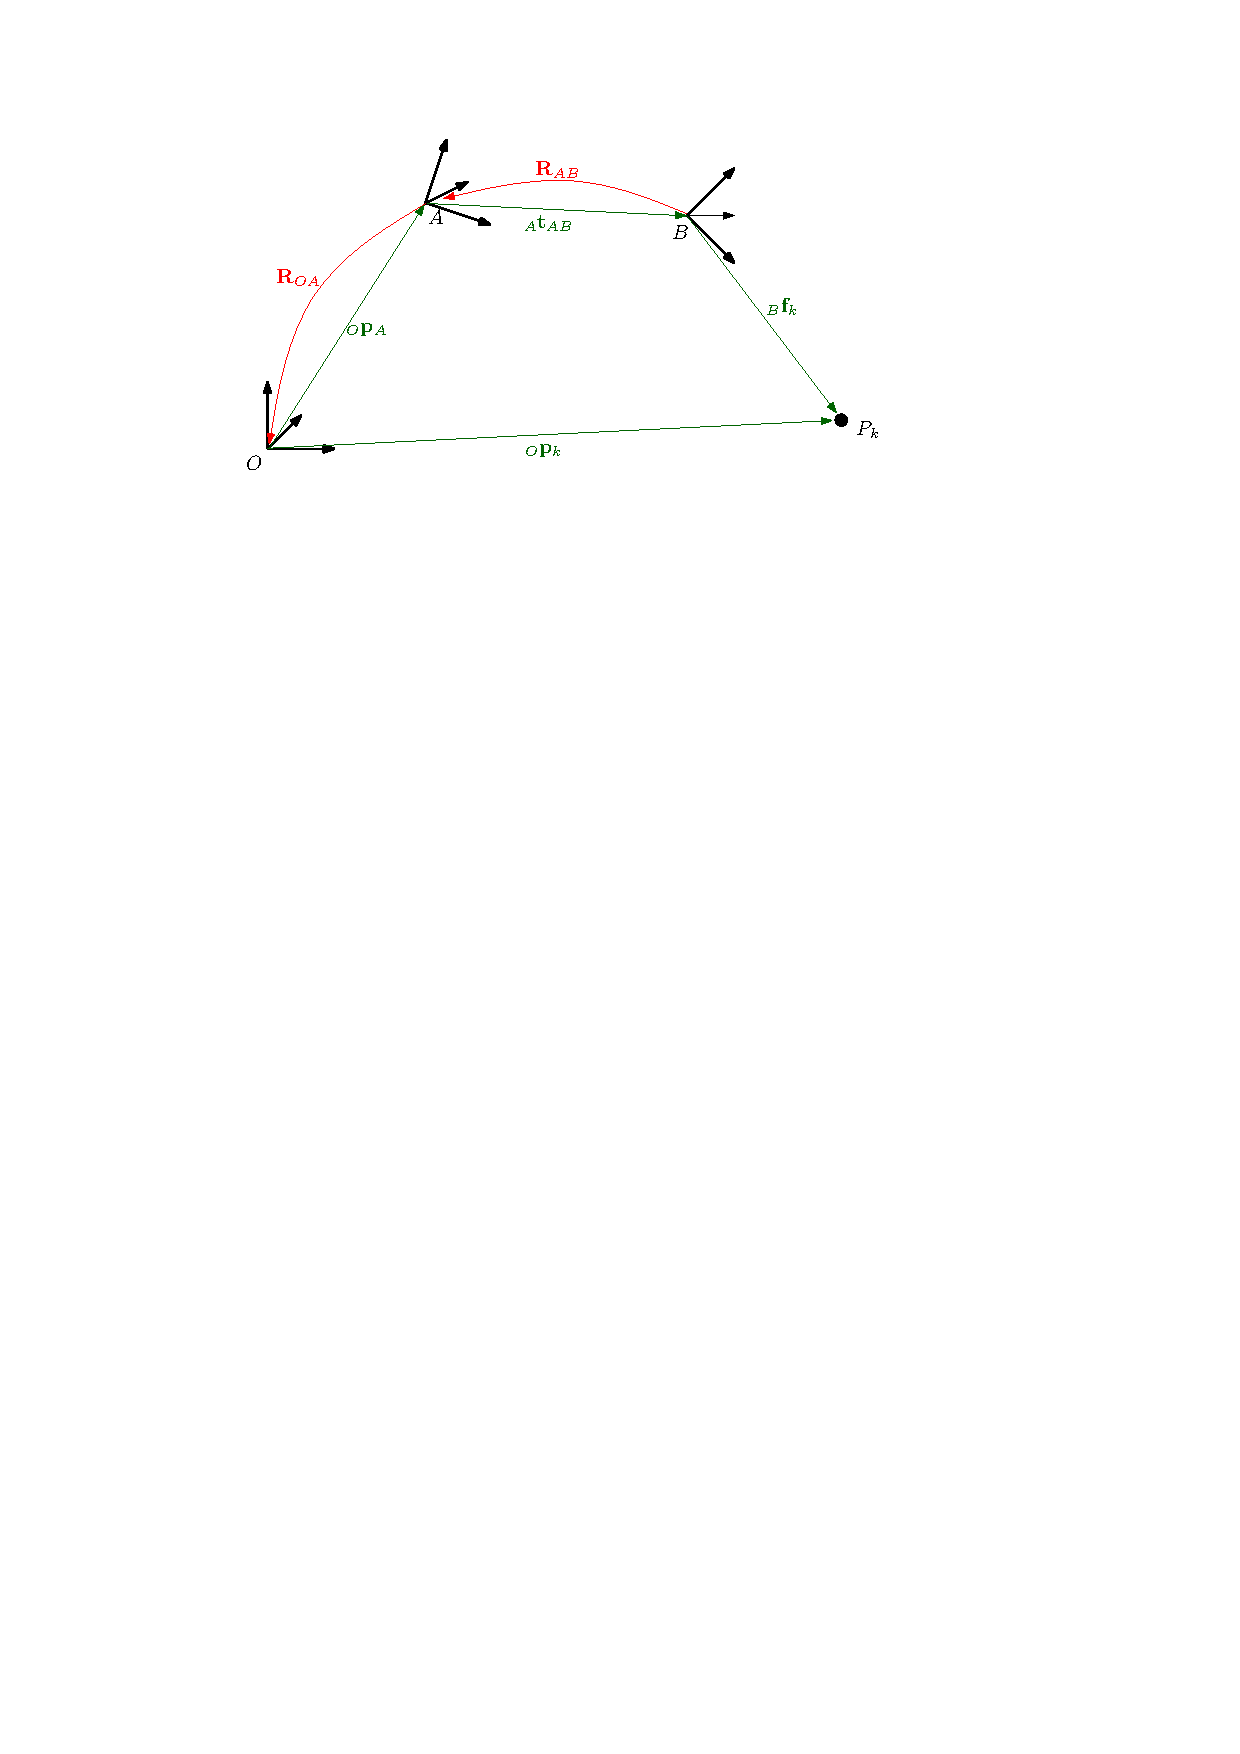
\includegraphics[width=0.6\textwidth]{img/notation.pdf}
     \caption{Example of a figure.}
     \label{img:notation}
  \end{figure}


\section{Including Code in your Document}

  You may include samples from your Matlab code using the \texttt{lstlistings} environment, for example
  \lstset{language=Matlab,numbers=none}
  \begin{lstlisting}[frame=lines, caption=Matlab Example, label=matlabexample]
  % Evaluate y = 2x
  for i = 1:length(x)

    y(i) = 2*x(i);

  end
  \end{lstlisting}

  \lstset{language=C++,numbers=none,caption=C++ Example, label=cppexample}
  \begin{lstlisting}[frame=lines]
  % sum all elements in a list
  int sum=0;
  for(list<int>::iterator it=mylist.begin(); it!=mylist.end(); ++it)
    sum += *it;
  \end{lstlisting}